\documentclass{article}
\usepackage[utf8]{inputenc}
\usepackage{listings}
\usepackage{amsfonts}
\lstset{
	language=Octave,
	frame=single,
	xleftmargin=.1\textwidth, xrightmargin=.1\textwidth
}
\usepackage{graphicx}
\usepackage{mathtools, nccmath}
\usepackage[T2A]{fontenc}
\usepackage[utf8]{inputenc}
\usepackage[russian]{babel}
\usepackage[left=2cm,right=2cm,top=2cm,bottom=2.1cm,bindingoffset=0cm]{geometry}

\graphicspath{{/pic}}
\DeclarePairedDelimiter{\nint}\lfloor\rfloor


\title{Упражнения из учебника}
\author{Кокорин Илья, M3439}

\begin{document}
	\maketitle
	\section{Упражнение 2.12}
	\subsection{А}
	Линейное пространство имеет вид $\{00,01,10,11\}$
	
	Базис имеет вид $\{10,01\}$, так как эти вектора линейно независимы, а любой другой может быть получен их комбинацией.
	
	Тогда $
	G = \left(
	\begin{array}{cccccccccc}
	1 & 0\\
	0 & 1
	\end{array}
	\right)
	$
	
	В этом случае, $n = 2, k = 2$
	
	Тогда $r = n - k = 2 - 2 = 0$, то есть матрица $H$ имеет размерность $0 \times 2$, то есть проверочная матрица не определена.
	
	\subsection{Б}
	Линейное пространство имеет вид $\{000,001,010,011,100,101,110,111\}$
	
	Базис имеет вид $\{100, 010, 001\}$, так как эти вектора линейно независимы, а любой другой может быть получен их комбинацией.
	
	Тогда $
	G = \left(
	\begin{array}{cccccccccc}
	1 & 0 & 0\\
	0 & 1 & 0\\
	0 & 0 & 1
	\end{array}
	\right)
	$
	
	В этом случае, $n = 3, k = 3$
	
	Тогда $r = n - k = 3 - 3 = 0$, то есть матрица $H$ имеет размерность $0 \times 3$, то есть проверочная матрица не определена.
	
	\subsection{В}
	Линейное пространство имеет вид $\{000,011,101,110\}$
	
	Базис имеет вид $\{101, 110\}$, так как эти вектора линейно независимы, а любой другой может быть получен их комбинацией.
	
	Тогда $
	G = \left(
	\begin{array}{cccccccccc}
	1 & 0 & 1\\
	1 & 1 & 0
	\end{array}
	\right)
	$
	
	Приведём $G$ к виду $(I_k, P)$
	
	$
	\left(
	\begin{array}{cccccccccc}
	1 & 0 & 1\\
	1 & 1 & 0
	\end{array}
	\right)
	$
	
	Заменяем вторую строку на линейную комбинацию второй и первой
	
	$
	\left(
	\begin{array}{cccccccccc}
	1 & 0 & 1\\
	0 & 1 & 1
	\end{array}
	\right)
	$
	
	Тогда $
	P = \left(
	\begin{array}{cccccccccc}
	1\\
	1
	\end{array}
	\right)
	$
	
	Тогда $
	P^T = \left(
	\begin{array}{cccccccccc}
	1 & 1
	\end{array}
	\right)
	$
	
	$H = (P^T, I_r) =  \left(
	\begin{array}{cccccccccc}
	1 & 1 & 1
	\end{array}
	\right)$
	
	Проверка показывает, что $G \cdot H^T = 0$
	
	\subsection{Г}
	Линейное пространство имеет вид $\{000,111\}$
	
	Базис имеет вид $\{111\}$, так как $000 = 0 \cdot 111$
	
	Тогда $
	G = \left(
	\begin{array}{cccccccccc}
	1 & 1 & 1
	\end{array}
	\right)
	$
	
	Тогда $P = \left(
	\begin{array}{cccccccccc}
	1 & 1
	\end{array}
	\right)$
	
	Тогда $P^T = \left(
	\begin{array}{cccccccccc}
	1\\
	1
	\end{array}
	\right)$
	
	Тогда $H = \left(
	\begin{array}{cccccccccc}
	1 & 1 & 0\\
	1 & 0 & 1
	\end{array}
	\right)$
	
	Проверка показывает, что $G \cdot H^T = 0$
	
	\section{Упражнение 1.3.}
	
	\subsection{Код из упражнения 1.1.}
	
	Каждый бит передаётся три раза. То есть если по каналу мы хотели передать бит 0, будет передана последовательность 000, а если хотели передать бит 1, будет передана последовательность 111.
	
	Следовательно, декодер выдаёт ошибку, если три бита неодинаковые. Значит, ошибка произошла либо в одном бите, либо в двух. 
	
	Так как мы используем двоичный симметричный канал, то вероятность ошибки в каждом бите это случайная величина Бернулли с вероятностью инвертирования бита $p$, и отсутствия инвертирования $1 - p$. Значит, для подсчёта вероятности ошибки в одном или двух битах мы можем использовать биномиальное распределение, являющееся суммой распределений Бернулли.
	
	Посчитаем вероятность ошибки строго в двух битах, воспользуемя биномиальным распределением
	
	$P_2 = C^2_3 \cdot p^2 \cdot (1 - p) = 3 \cdot p^2 \cdot (1 - p) $
	
	Аналогично посчитаем вероятность ошибки в одном бите 
	$P_1 = C^1_3 \cdot p \cdot (1 - p)^2 = 3 \cdot p \cdot (1 - p)^2 $
	
	Тогда вероятность того, что декодер выдаст ошибку (то есть произойдёт инверсия двух или одного бита) равна $P = P_1 + P_2 = 3 \cdot p \cdot (1 - p)^2 +  3 \cdot p^2 \cdot (1 - p)$, что при $p = 10^{-3}$ равно $\frac{2997}{1000000}$
	
	Для того, чтобы пользователь получил ложную информацию, инвертироваться должны все три бита (то есть из 000 должен получиться 111, а из 111 должен получиться 000), тогда декодер выдаст неверную информацию. Посчитаем вероятность инверсии в трёх из трёх битов, при условии, что инверсия каждого бита независима. Она равна $P = p^3 = (10^{-3})^{-3} = 10^{-9}$
	
	\subsection{Код из упражнения 1.2}
	
	Заметим, что при передаче может быть инвертировано от одного до пяти бит.
	
	При этом $k$ бит можно инвертировать $C^k_5$ способами.
	
	\begin{center}
		\begin{tabular}{cc}
			$k$: & $C^k_5$ \\
			$1$: & $5$\\
			$2$: & $10$ \\
			$3$: & $10$ \\
			$4$: & $5$ \\
			$5$: & $1$  \\
		\end{tabular}
	\end{center}
	
	Запишем кодовые слова и выясним, сколько  бит нужно в инвертировать в каждом из них, чтобы попасть в какое-то другое слово (то есть чтобы декодер выдал не ошибку декодировки, а неправильно декодировал)
	
	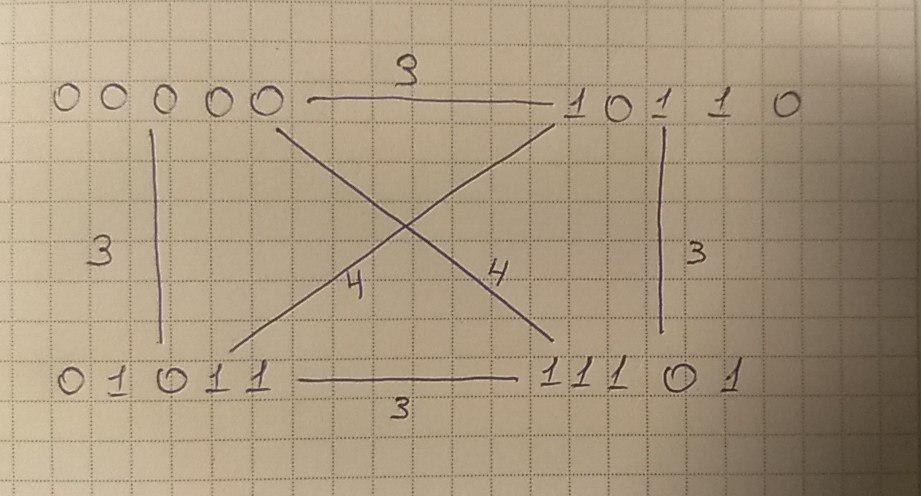
\includegraphics[scale=0.5]{pic/pic-1.jpg}
	
	Заметим, что из каждого кодового слова можно попасть в другое кодовое слово либо одной из двух трёхсимвольных замён, либо единственной четырёхсимвольной замёной. То есть у нас есть: 5 односимвольных замен, из которых ни одна не приводит в другое кодовое слово, 10 двухсимвольных замен, из которых ни одна не приводит в другое кодовое слово, 10 трёхсимвольных замен, из которых 2 приводят в другое кодовое слово, а 8 не приводят, 0 четырёхсимвольных замен, из которых 1 приводит в другое кодовое слово, а 4 не приводят, и 1 пятисимвольная замена, не приводящее в другое слово.
	
	\begin{center}
		\begin{tabular}{ccc}
			$k$: & число замен, приводящих к другому кодовому слову & число замен, приводящих к ошибке \\
			$1$: & $0$ & $5$\\
			$2$: & $0$ & $10$ \\
			$3$: & $2$ & $8$\\
			$4$: & $1$ & $4$ \\
			$5$: & $0$ & $1$  \\
		\end{tabular}
	\end{center}

	Значит, вероятностью выдачи декодером ошибки будет $P^{err} = P^{err}_1 + P^{err}_2 + P^{err}_3 + P^{err}_4 + P^{err}_5 = 5 \cdot p \cdot (1 - p)^4 + 10 \cdot p^2 \cdot (1 - p)^3 + 8 \cdot p^3 \cdot (1 - p)^2 + 4 \cdot p^4 \cdot (1 - p) + 1 \cdot p^5 = \frac{2495003999}{500000000000} = 0.00499001$
	
	Тогда вероятность выдачи декодером неверного сигнала будет $P^{wrong} = P^{wrong}_1 + P^{wrong}_2 + P^{wrong}_3 + P^{wrong}_4 + P^{wrong}_5 = 2 \cdot p^3 \cdot (1 - p)^2 + 1 \cdot p^4 \cdot (1 - p) = \frac{1997001}{1000000000000000} = 1.997 \cdot 10^{-9}$
	
	\section{Задача 1.1}
	
	Запишем расстояние Хеминга в виде
	
	$\rho(a, b) = \sum\limits_{i = 1}^n |a_i \neq b_i|$, то есть количество позиций, в которых $a$ и $b$ отличаются.
	
	\subsection{Неотрицательность}
	
	Очевидно, $\rho(a, b) \geq 0$, так как две строки отличаются в неотрицательном числе позиций.
	
	\subsection{Симметричность}
	
	$\rho(a, b) = \sum\limits_{i = 1}^n |a_i \neq b_i| = \sum\limits_{i = 1}^n |b_i \neq a_i| = \rho(b, a)$
	
	\subsection{Неравенство треугольника}
	
	Докажем, что $\rho(a, b) \leq \rho(a, c) + \rho(b, c)$
	
	То есть докажем $\sum\limits_{i = 1}^n |a_i \neq b_i|  \leq \sum\limits_{i = 1}^n |a_i \neq c_i| + \sum\limits_{i = 1}^n |c_i\neq- b_i|  = \sum\limits_{i = 1}^n (|a_i \neq b_i| + |c_i \neq b_i|)$
	
	Пусть $a$ отличается от $b$ в некоторой позиции $i$, то есть $|a_i \neq b_i| = 1$. Очевидно, что тогда $c$ будет отличаться в этой позиции либо от $a$, либо от $b$ ($c$ не может совпадать в этой позиции как с $a$, так и с $b$, так как $a$ и $b$ в этой позиции отличаются). Тогда
	
	$|a_i \neq b_i| = 1 \Rightarrow \left[
	\begin{array}{ccc}
	|a_i \neq c_i| = 1 \\
	|c_i \neq b_i| = 1\\
	\end{array}
	\right. \Rightarrow |a_i \neq b_i| + |c_i \neq b_i|  \geq  |a_i - b_i|$
	
	Если же $а$ не отличается от $b$ в некоторой позиции, то есть $|a_i \neq b_i| = 0$. Тогда в силу неотрицательности $|a_i \neq b_i| + |c_i \neq b_i|, |a_i \neq b_i| + |c_i \neq b_i| \geq |a_i \neq b_i|$
	
	Тогда $\forall i \in \{1..n\}: |a_i \neq b_i| + |c_i \neq b_i| \geq |a_i \neq b_i| \Rightarrow \sum\limits_{i = 1}^n |a_i \neq b_i|  \leq  \sum\limits_{i = 1}^n (|a_i \neq b_i| + |c_i \neq b_i|) = \sum\limits_{i = 1}^n |a_i \neq c_i| + \sum\limits_{i = 1}^n |c_i \neq b_i| \Rightarrow \rho(a, b) \leq \rho(a, c) + \rho(b, c)$
	
	\section{Задача 1.2}
	
	Чтобы декодирование по принципу максимального правдоподобия и паксимуму апостериорной вероятности были эквивалентными, необходимо соблюдение условия $\forall m \in \{1..M\}: P(y|c_m) = P(c_m|y)$
	
	$P(c_m|y) = \frac{P(c_m \& y)}{P(y)}$
	
	Заметим, что $P(y|c_m) = \frac{P(y \& c_m)}{P(c_m)} \Rightarrow P(y\& c_m) = P(y|c_m) \cdot P(c_m)$
	
	Тогда $P(c_m|y) = \frac{P(c_m\& y)}{P(y)} = \frac{P(y|c_m) \cdot P(c_m)}{P(y)} =$
	
	Распишем $P(y)$ по формуле полной вероятности.
	
	$= \frac{P(y|c_m) \cdot P(c_m)}{\sum\limits_{i = 1}^M P(y|c_i) \cdot P(c_i)}$
	
	Так как $P(y|c_m) = P(c_m|y)$, то $P(c_m|y)= \frac{P(y|c_m) \cdot P(c_m)}{\sum\limits_{i = 1}^M P(y|c_i) \cdot P(c_i)}$ превращается в 
	
	$1 = \frac{P(c_m)}{\sum\limits_{i = 1}^M P(y|c_i) \cdot P(c_i)} \Rightarrow P(c_m) = \sum\limits_{i = 1}^M P(y|c_i) \cdot P(c_i)$
	
	Значит, $\forall m \in \{1..M\}: c_m$ - константа, не зависящая от $m$. Тогда $\forall m \in \{1..M\}: c_m = \frac{1}{M}$, то есть кодовые слова должны быть распределены равновероятно.
	
	Проверим соблюдение требуемого условия при таком распределении кодовых слов:
	
	 $P(c_m|y)= \frac{P(y|c_m) \cdot P(c_m)}{\sum\limits_{i = 1}^M P(y|c_i) \cdot P(c_i)} = \frac{P(y|c_m) \cdot \frac{1}{M}}{\sum\limits_{i = 1}^M P(y|c_i) \cdot \frac{1}{M}} = \frac{P(y|c_m) \cdot \frac{1}{M}}{\frac{1}{M} \cdot \sum\limits_{i = 1}^M P(y|c_i)} = \frac{P(y|c_m)}{\sum\limits_{i = 1}^M P(y|c_i)} =  \frac{P(y|c_m)}{1} = P(y|c_m)$, что и требовалось доказать.
	 
	 \section{Задача 1.3}
	 
	 Запишем среднюю вероятность правильного декодирования в виде $P_c = \sum\limits_m P(c_m) \cdot \sum\limits_{y \in R_m} P(y|c_m)$, где $R_m$ - множество тех $y$, по которым принимается решение в пользу $c_m$.
	 
	 Заметим, что $1 - P_c = \sum\limits_y P(y) -  \sum\limits_m P(c_m) \cdot \sum\limits_{y \in R_m} P(y|c_m) = \sum\limits_y \sum\limits_m P(y|c_m) \cdot P(c_m) -  \sum\limits_m P(c_m) \cdot \sum\limits_{y \in R_m} P(y|c_m) = \sum\limits_m \sum\limits_y P(y|c_m) \cdot P(c_m) -  \sum\limits_m P(c_m) \cdot \sum\limits_{y \in R_m} P(y|c_m) = \sum\limits_m P(c_m) \cdot \sum\limits_y P(y|c_m) -  \sum\limits_m P(c_m) \cdot \sum\limits_{y \in R_m} P(y|c_m) = \sum\limits_{m} P(c_m) \cdot (\sum\limits_y P(y|c_m) - \sum\limits_{y \in R_m} P(y|c_m)) =  \sum\limits_{m} P(c_m) \cdot \sum\limits_{y \in T_m} P(y|c_m)$, где $T_m$ - множество тех $y$, по которым принимается решение не в пользу $c_m$, $ = \sum\limits_m P(c_m) \cdot P(\hat{m} \neq m| x = c_m) = P_e$, то есть $P_e = 1 - P_c$. То есть, максимизируя $P_c$, мы минимизируем $P_e$. Докажем теперь, что МАВ максимизирует $P_c$.
	 
	 $P_c = \sum\limits_m P(c_m) \cdot \sum\limits_{y \in R_m} P(y|c_m) = \sum\limits_m \sum\limits_{y \in R_m} P(y|c_m) \cdot P(c_m) = \sum\limits_m \sum\limits_{y \in R_m} \frac{P(y \& c_m)}{P(c_m)} \cdot P(c_m) = \sum\limits_m \sum\limits_{y \in R_m} P(y \& c_m) = \sum\limits_m \sum\limits_{y \in R_m} \frac{P(y \& c_m)}{P(y)} \cdot P(y) = \sum\limits_m \sum\limits_{y \in R_m} P(c_m|y) \cdot P(y)$
	 
	 Так как декодирование по МАВ максимизирует $P(c_m|y)$, значит, максимизироваться будет каждое слагаемое суммы, а значит, и вся сумма также будет максимизироваться. Значит, максимизироваться будет $P_c = 1 - P_e$, а значит, $P_e$ будет минимизироваться.
	 
	 \section{Задача 1.4}
	 
	 Пусть $a$ - переданное слово, $b$ - полученное. Длины этих слов равны $n$.
	 Посчитаем $P(b|a)$. 
	 
	 Пусть $d(a, b) = d$. То есть a и b отличаются в d позициях и совпадают в $n - d$ позициях.
	 
	 Тогда $P(b|a) = \prod\limits_{i = 1}^n P(b_i|a_i)$
	 
	 При этом $d$ из этих множителей будут равны $\frac{p_0}{q - 1}$, а $n - d$ множителей равны $1 - p_0$
	 
	 Тогда $P(b|a) = \prod\limits_{i = 1}^n P(b_i|a_i) = (\frac{p_0}{q - 1})^d \cdot (1 - p_0)^{n - d} = (\frac{p_0}{q - 1})^d \cdot \frac{(1 - p_0)^n}{(1 - p_0)^d} = (\frac{p_0}{q - 1})^d \cdot \frac{1^d}{(1 - p_0)^d} \cdot (1 - p_0)^n =(\frac{p_0}{q - 1})^d \cdot (\frac{1}{1 - p_0})^d \cdot (1 - p_0)^n = (\frac{p_0}{(q - 1) \cdot (1 - p_0)})^d \cdot (1 - p_0)^n $
	 
	 Так как $(1 - p_0)^n$ является константой, минимизация $P(b|a)$ эквивалетна минимизации $(\frac{p_0}{(q - 1) \cdot (1 - p_0)})^d$ 
	 
	 Минимизация $(\frac{p_0}{(q - 1) \cdot (1 - p_0)})^d$ эквивалентна максимизации $d$, если $0 < \frac{p_0}{(q - 1) \cdot (1 - p_0)} < 1$
	 
	 Так как $p_0 \in (0; 1)$, то $1 - p_0 \in (0; 1)$
	 
	 Так как $q > 1$, то $q - 1 > 0$
	 
	 Значит, $(q - 1) \cdot (1 - p_0) > 0$, и $\frac{p_0}{(q - 1) \cdot (1 - p_0)} > 0$ всегда. 
	 
	 Значит, найдём такие значения параметров, при которых $\frac{p_0}{(q - 1) \cdot (1 - p_0)} < 1$
	 
	 $p_0 < (q - 1) \cdot (1 - p_0)$
	 
	  $p_0 < q - q \cdot p_0 - 1 + p_0$
	  
	  $q - q \cdot p_0 - 1 > 0$
	  
	  $q \cdot (1 - p_0) > 1$
	  
	  $q > \frac{1}{1 - p_0}$
	  
	  Итого, $p_0 \in (0; 1) \& q > \frac{1}{1 - p_0}$ даёт эквивалентность декодирования по минимизации расстояних Хемминга и декодирования по МП.
	  
	  \section{Задача 1.5}
	  
	  \subsection{Исправление ошибок}
	  Пусть a - переданное слово, b - принятое слово. Пусть $d(a, b) = t$. Мы хотим, чтобы декодер сопоставил принятому слову b слово a, которое передавалось исходно.
	  
	  Для этого необходимо чтобы $\forall c \neq a: d(c, b) > d(a, b)$, так как в противном случае вместо слова a, которое было передано по каналу, декодер выберет слово $c \neq a$, что приведёт к неправильной декодировке.
	  
	  Тогда $\forall c \neq a: d(c, b) > t \Rightarrow min_{c \neq a} d(c, b) \geq t + 1$
	  
	  Тогда минимальное расстояние между различными кодовыми словами $a \neq c$ должно быть не меньше $2t + 1$. Тогда $d \geq 2t + 1 \Rightarrow 2t + 1 \leq d \Rightarrow 2t \leq d - 1 \Rightarrow t \leq \frac{d - 1}{2}$. Учитывая тот факт, что $t \in \mathbb{N}$, получаем $t \leq \nint{\frac{d - 1}{2}}$
	  
	  \subsection{Выявление ошибок}
	  
	  Пусть а - переданное слово, b - принятое слово, $d(a, b) = t$. Если принятое слово b не является кодовым, то декодер может сообщить об ошибке. Для обнаружения ошибки слово b не должно оказаться кодовым, значит, не должно существовать кодовых слов на расстоянии t. Значит, $\forall a \neq b: d(a, b) > t \Rightarrow d > t \Rightarrow d \geq t + 1 \Rightarrow t \leq d - 1$. 
	  
	  \subsection{Геометрическое обоснование}
	  
	  Этим фактам есть и простое геометрическое обоснование. Введём понятие шара $R_t(a) = \{b: d(a, b) < t\}$ - все  слова, находящиеся от данного на расстоянии строго меньше t.
	  
	  Тогда если минимальное расстояние кода равно $d$, то $min_{a \neq b} d(a, b) = d$, значит, в шаре радиуса d - 1,построенном вокруг кодового слова a, нет других кодовых слов. 
	  
	  Значит, совершив не более $d - 1$ ошибок при передаче кодового слова a, мы попадаем в шар $R_{d - 1}(a)$, построенный вокруг передаваемого кодового слова a. Известно, что в этом шаре нет других кодовых слов, поэтому мы можем сообщить об ошибке.
	  
	  Очевидно, что $\forall a \neq b: R_{\nint{\frac{d - 1}{2}}}(a) \cap R_{\nint{\frac{d - 1}{2}}}(b) = \emptyset$. Значит, совершив не более $\nint{\frac{d - 1}{2}}$ ошибок при передаче кодового слова a, мы попадаем в шар $R_{\nint{\frac{d - 1}{2}}}(a)$, построенный вокруг передаваемого кодового слова a. Известно, что этот шар не пересекается ни с одним из других шаров, а значит, мы можем брать ближайшее кодовое слово. Этим кодовым словом является a, так как мы лежим в шаре радиуса $\nint{\frac{d - 1}{2}}$, построенном вокруг него, и не лежим ни в одном из шаров радиуса $\nint{\frac{d - 1}{2}}$, построенном вокруг других кодовых слов. 
\end{document}